\documentclass[10pt,a4paper]{article}
\usepackage[a4paper,margin=22mm]{geometry}
\usepackage[T1]{fontenc}
\usepackage{palatino}
\usepackage{xcolor}
\usepackage{hyperref}
\usepackage{enumitem}
\usepackage{tabularx}
\usepackage{array}
\usepackage{graphicx}
\definecolor{navy}{HTML}{17365D}
\setlist[itemize]{leftmargin=1.3em,noitemsep,topsep=3pt}
\setlength{\parindent}{0pt}
\begin{document}
{\Large\bfseries\color{navy} Dynamic Receptive Fields in Mouse Auditory Cortex}\par\vspace{4pt}
{\small Xuan Li Feng \quad | \quad Imperial College London \quad | \quad 2025--2026}\par\vspace{12pt}
\hrule\vspace{12pt}
\textbf{Technical project brief}\par
\vspace{3pt}
This project evaluated whether a dynamic receptive-field model could predict auditory-cortical activity from natural ultrasonic vocalisations and recover response properties missed by static methods.
\section*{Research question}
Can a stimulus-dependent receptive field capture nonlinear neural-response behaviour not represented by conventional static receptive-field methods?
\section*{Analysis architecture}
\[
\mbox{Natural sound spectrograms} \;\longleftrightarrow\; \mbox{Causal Conv1D model} \;\longleftrightarrow\; \mbox{Dynamic STRF extraction}
\]
\section*{Implemented analysis}
\begin{itemize}
\item Trained a five-layer causal Conv1D model in PyTorch on sound spectrograms from 46 mouse auditory-cortex units.
\item Used Jacobian-based automatic differentiation to derive dynamic spectrotemporal receptive fields from the trained network.
\item Compared the model with spike-triggered average, spike-triggered covariance, and maximum-noise-entropy baselines.
\item Evaluated held-out firing-rate prediction with Pearson correlation, matched comparison protocols, and shuffle tests.
\end{itemize}
\section*{Analysis map}
\renewcommand{\arraystretch}{1.5}
\begin{tabularx}{\linewidth}{>{\bfseries\color{navy}}p{0.29\linewidth}X}
Input & Natural ultrasonic vocalisations represented as spectrograms \\
Prediction model & Causal Conv1D network producing firing-rate predictions \\
Response analysis & Jacobian-based extraction of dynamic receptive-field structure \\
Evaluation & Held-out Pearson correlation, matched comparisons, shuffle tests, and temporal-hold analysis \\
\end{tabularx}
\section*{Project outcome}
The dynamic STRF achieved a median held-out Pearson correlation of \textbf{0.339} and revealed temporal hold in \textbf{43.5\%} of analysed neurons. Under matched settings, the dynamic model outperformed the static alternatives and supported context-dependent analysis of neural responses to naturalistic sound.
\section*{Technical tools}
PyTorch \quad Python \quad Conv1D \quad Automatic differentiation \quad Spectrotemporal analysis \quad Statistical model comparison
\vfill
{\small\color{navy}\rule{0.12\linewidth}{0.5pt}\quad Public project summary}

\newpage
{\Large\bfseries\color{navy} Selected results}\par\vspace{4pt}
{\small Dynamic receptive-field modelling in mouse auditory cortex}\par\vspace{10pt}
\hrule\vspace{12pt}
\textbf{Prediction example}\par\vspace{5pt}
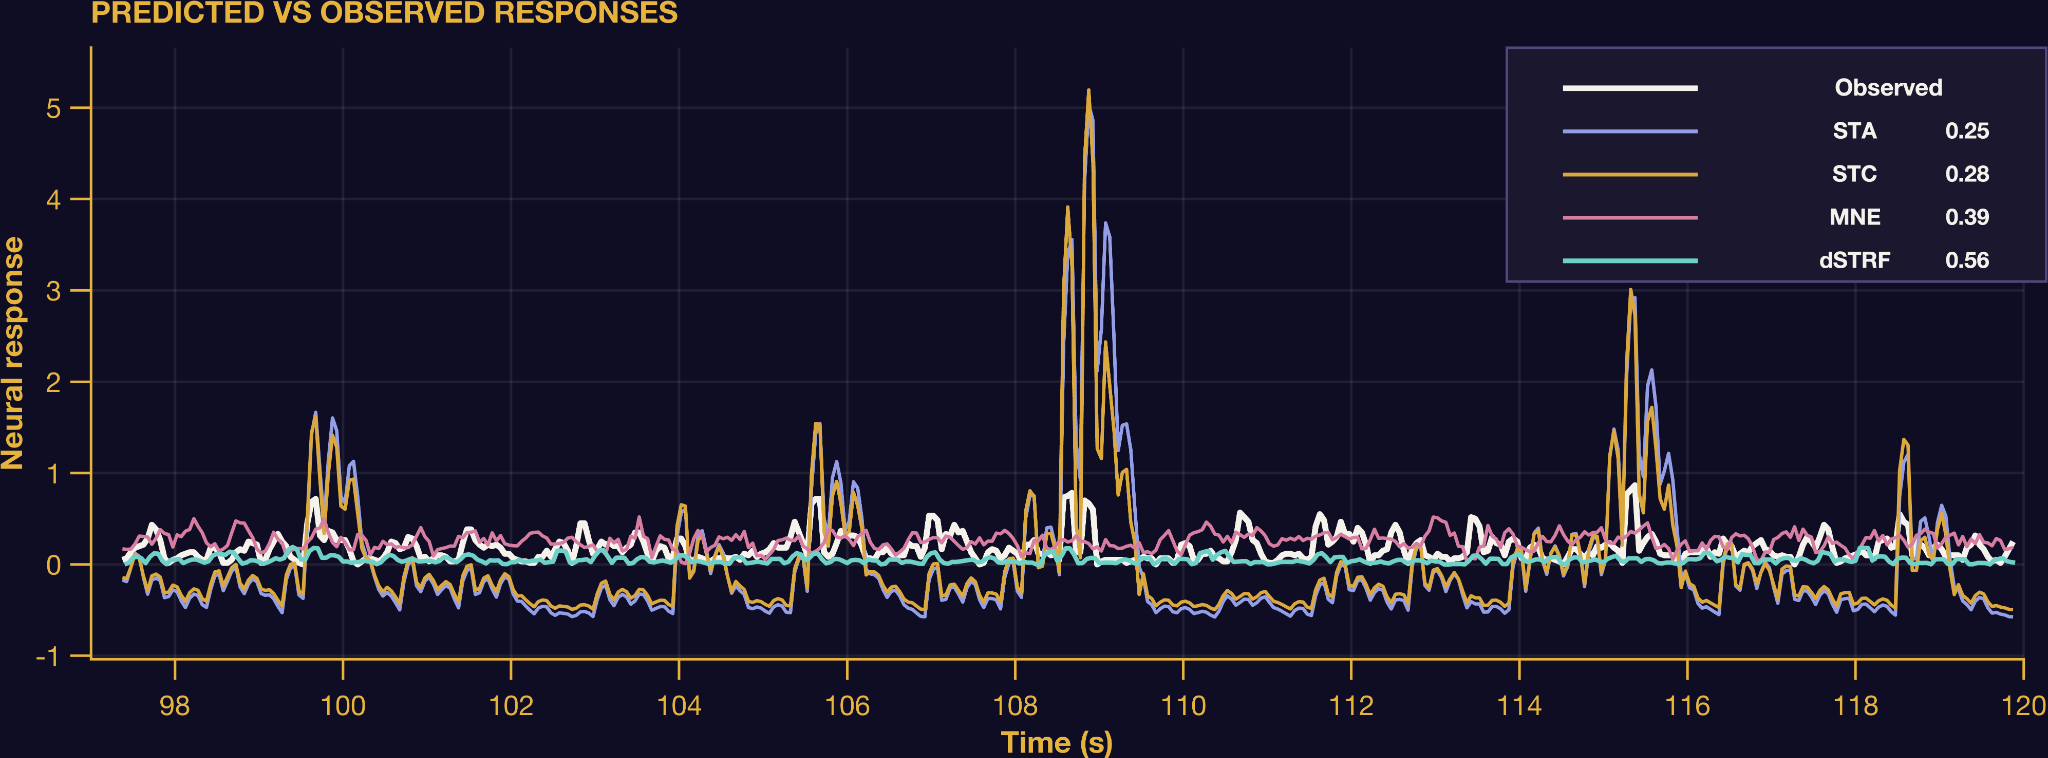
\includegraphics[width=\linewidth]{assets/neural_prediction_comparison.png}\par
\vspace{4pt}
{\small A representative segment comparing observed neural activity with predictions from STA, STC, MNE, and dynamic STRF methods.}\par\vspace{12pt}
\textbf{Performance across 46 neurons}\par\vspace{5pt}
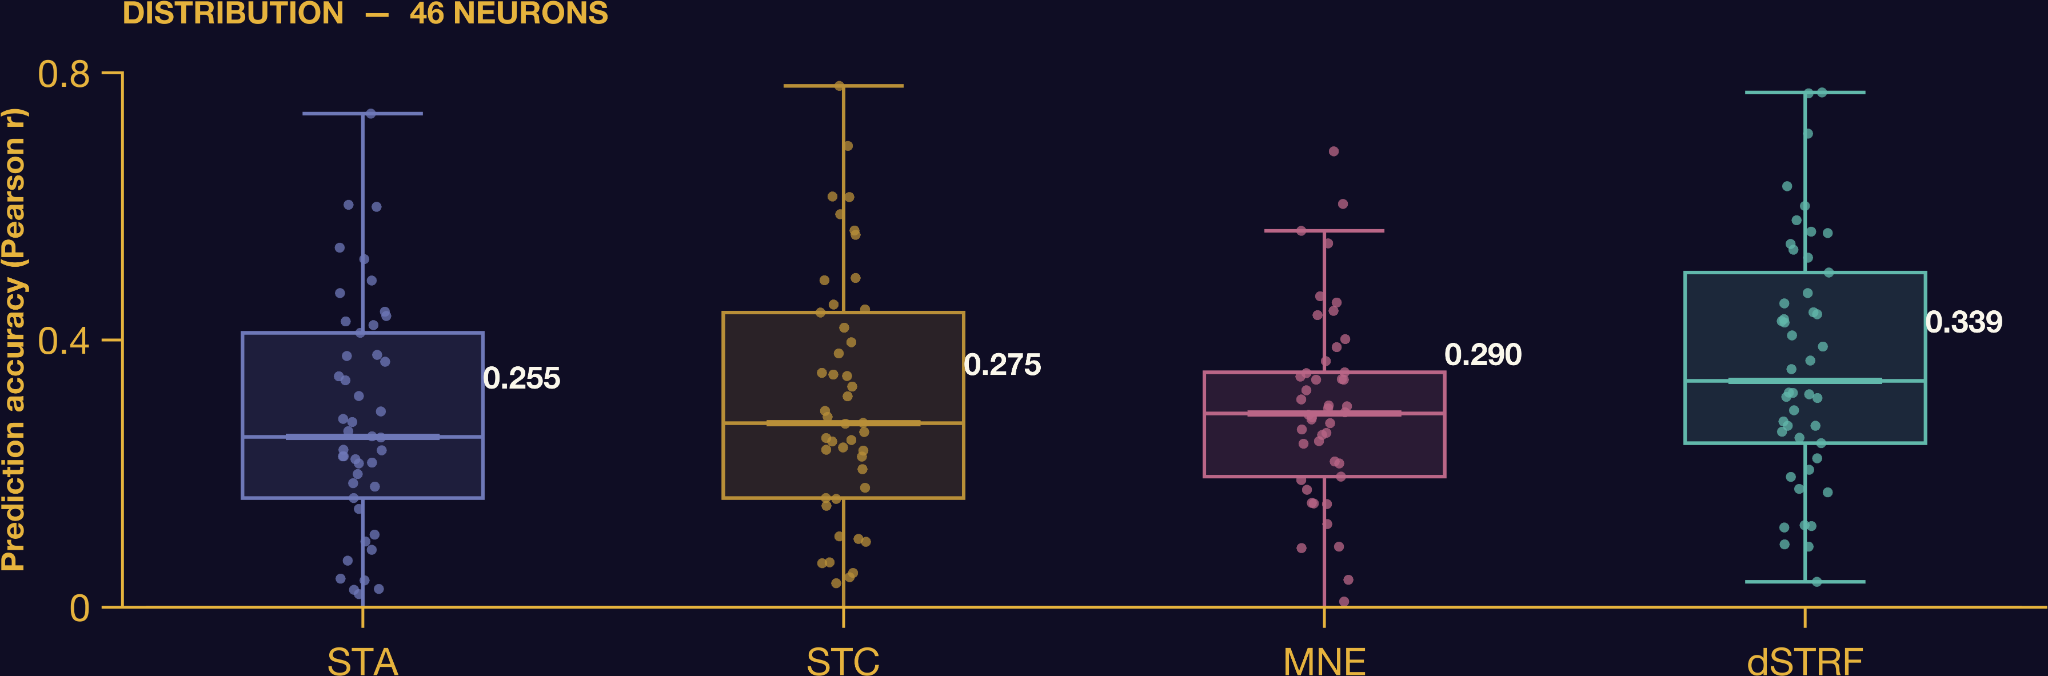
\includegraphics[width=\linewidth]{assets/neural_method_comparison.png}\par
\vspace{4pt}
{\small The dynamic STRF model achieved the highest median prediction accuracy across the evaluated population.}
\end{document}
